\section{Ethernet und LAN}
\subsection{Local Area Networks (LAN)}

\begin{definition}{LAN}\\
    Räumlich kleines Netzwerk mit hoher Geschwindigkeit
    \begin{itemize}
        \item 10 m .. wenige km
        \item 100 Mbps .. 100 Gbit/s, typisch heute 1 Gbit/s
    \end{itemize}
    Verbindet Server, Workstations, PCs, Drucker, NAS, …
    \begin{itemize}
        \item Auf Schicht 2 (direkte Kommunikation zwischen allen Stationen innerhalb des LAN)
    \end{itemize}
    Vorteile/Möglichkeiten:
    \begin{itemize}
        \item Gemeinsamer Zugriff (Drucker)
        \item Datenaustausch (Directory/File Sharing)
        \item Direkte Kommunikation (VoIP, Gaming)
        \item Zugang zum Internet (über einen Router im LAN)
    \end{itemize}
\end{definition}

\subsubsection{Topologien}

\begin{definition}{Bus}
    \begin{itemize}
        \item Alle Stationen
        \begin{itemize}
            \item sind passiv angeschlossen
            \item horchen Leitung permanent ab
            \item werden aktiv, wenn sie etwas senden wollen
        \end{itemize}
        \item Keine festgelegte Ausbreitungsrichtung
        \item Empfänger erkennt anhand einer Adresse, ob die Daten für ihn relevant sind
    \end{itemize}
\end{definition}

 
    \centering
    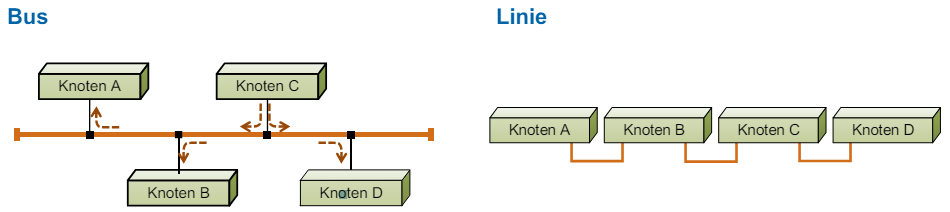
\includegraphics[width=1\linewidth]{images/bus_linie_topo.png}
 

\begin{definition}{Linien}
    \begin{itemize}
        \item Punkt-zu-Punkt Verbindungen zwischen benachbarten Knoten
        \item Alle Stationen müssen
        \begin{itemize}
            \item Daten empfangen
            \item Daten regenerieren
            \item falls nötig weiterleiten
        \end{itemize}
        \item Der Ausfall einer Station führt zur Segmentierung des LAN in zwei Teile
    \end{itemize}
\end{definition}

\begin{definition}{Ring}
    \begin{itemize}
        \item Benötigt Verfahren zur Verhinderung von «endlosem Kreisverkehr»
        \item Gewisse Redundanz: beim Ausfall einer Station kann immer noch jede Station erreicht werden
    \end{itemize}
\end{definition}

 
    \centering
    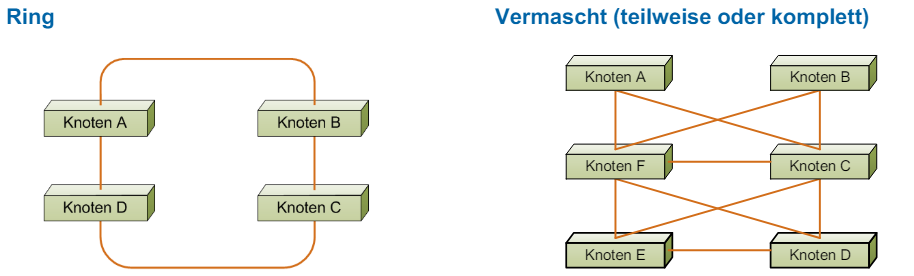
\includegraphics[width=1\linewidth]{images/ring_vermascht_topo.png}
 

\begin{definition}{Vermascht}
    \begin{itemize}
        \item Weitere Erhöhung der Redundanz:
        \begin{itemize}
            \item Ausfall einer oder eventuell auch mehrerer Stationen oder Verbindungen kann toleriert werden
            \item Zusätzliche Kosten und Aufwand, um mehrfache Lieferung von Daten zu verhindern
        \end{itemize}
    \end{itemize}
\end{definition}

\begin{definition}{Stern}
\begin{itemize}
    \item Jede Station an zentralen Verteiler (Switch/Bridge) angeschlossen
    \item Verteiler entkoppelt Knoten elektrisch und macht LAN weniger störungsanfällig
    \item Verteiler sendet Daten, die er von einer Station erhält, an die anderen Knoten weiter
\end{itemize}
\end{definition}

 
    \centering
    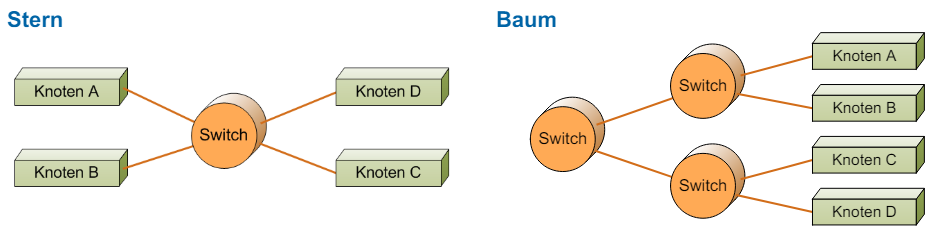
\includegraphics[width=1\linewidth]{images/stern_baum_topo.png}
 

\begin{definition}{Baum}
    \begin{itemize}
        \item Hierarchische Erweiterung der Sterntopologie
        \item Intelligenten Switches ermöglichen einen Grossteil der Kommunikation „lokal“
        \begin{itemize}
            \item zwischen A und B bzw. C und D
        \end{itemize}
        \item Dadurch Verringerung der Last für die einzelnen Switches
    \end{itemize}
\end{definition}

\subsubsection{Übertragung und Adressierung}

\begin{definition}{Übertragungsarten}\\
    In jedem Fall: genau 1 Sender
    \begin{itemize}
        \item Unicast:
        \begin{itemize}
            \item Genau ein, klar spezifizierter Empfänger
            \item Frame trägt die Adresse dieses Empfängers
            \item Analogie: Briefpost
        \end{itemize}
        \item Multicast:
        \begin{itemize}
            \item Eine Gruppe von Empfängern
            \item Frame trägt die Multicast-Adresse der Gruppe
            \item Analogie: Mailing-Liste
        \end{itemize}
        \item Broadcast:
        \begin{itemize}
            \item An alle Knoten im LAN gerichtet
            \item Frame trägt die Broadcast-Adresse des LAN
            \item Analogie: Radio-Sendestation
        \end{itemize}
    \end{itemize}
        \includegraphics[width=0.2\linewidth, angle=90]{images/übertragungsarten.png}\\
        Diese Begriffe werden nicht nur im LAN, sondern auch allgemein in Netzwerken verwendet
\end{definition}

\begin{concept}{Adressierung in LANs}
    \begin{itemize}
        \item Jede Station kann Daten von jeder anderen Station direkt empfangen
        \item Um zu erkennen, ob empfangene Daten für die eigene Station bestimmt sind, und wer der Absender ist, müssen die Adressen im LAN eindeutig sein.
        \item IEEE MAC Adressen
        \begin{itemize}
            \item werden nicht konfiguriert
            \item sind fix einem Interface des Gerätes zugeordnet
            \item bestehen aus 6 Bytes
            \item Darstellung hexadezimal 1A-2B-3C-4E-5F-67
        \end{itemize}
        \item Geräte sind möglicherweise mobil und wechseln zwischen LANs, oder LANS werden direkt verbunden $\longrightarrow$ Leitungscode
    \end{itemize}
\end{concept}

\begin{concept}{Manchester Leitungscode (10BASE-T)}\\
    Es wird ein Manchester-Code gesetzt:
    \begin{itemize}
        \item 1 positive Flanke, 0 negative Flanke
        \item Bei jedem Bit gibt es einen Signalwechsel
        \item Erlaubt die Taktrückgewinnung auf einfache Weise
        \item Bandbreite von 10 MHz benötigt (also das doppelte des theoretischen Minimums)
    \end{itemize}
        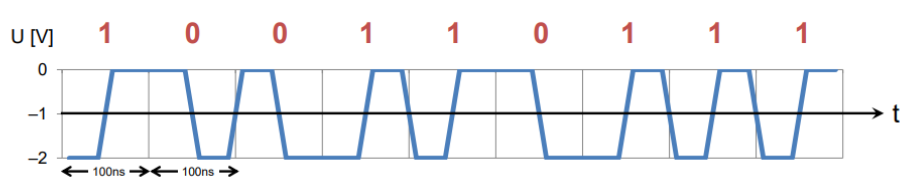
\includegraphics[width=0.8\linewidth]{images/leitungscode.png}
\end{concept}

\begin{definition}{Ethernet Format}
    Length/Type (2 Bytes)
    \begin{itemize}
        \item Fall 1: Länge von DATA ohne PAD ($\leq$ 1500)
        \item Fall 2: Typ von Data = Protokoll der nächsten Schicht ($\leqq$ 1536)
    \end{itemize}
    Data / Padding (46 – 1500 Bytes)
    \begin{itemize}
        \item Enthält die eigentlichen Datenbytes
        \item Bei weniger als 46 Bytes wird mit PAD Bytes abgefüllt
    \end{itemize}
    Frame Check Sequence, FCS (4 Bytes)
    \begin{itemize}
        \item IEEE CRC-32 Algorithmus
    \end{itemize}
    Interframe Gap, IFG (12 Bytes)
    \begin{itemize}
        \item «Zwangspause» zwischen aufeinanderfolgenden Frames
        \item Ist NICHT Teil des Ethernet Frames
    \end{itemize}
    \vspace{2mm}
            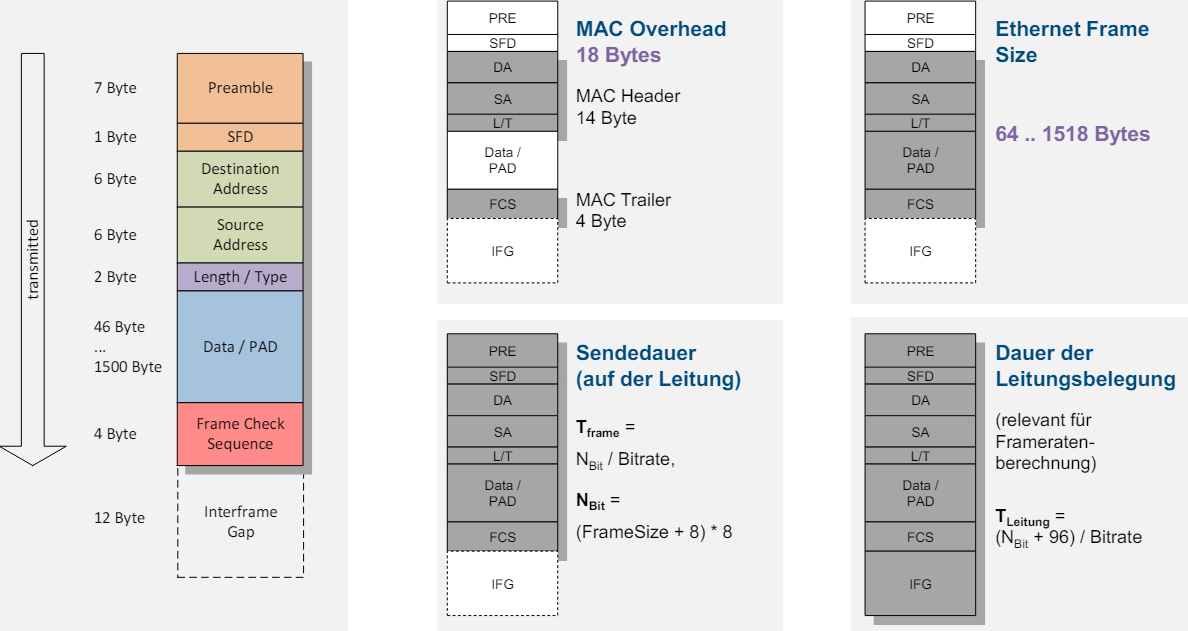
\includegraphics[width=1\linewidth]{images/ethernet_format.png}
\end{definition}

\begin{formula}{IEEE MAC Adressen}\\
    Registrierung bei IEEE:
    \begin{itemize}
        \item 3-Byte «OUI» identifiziert Hersteller
        \item 3-Byte Laufnummer durch Hersteller verwaltet
    \end{itemize}
        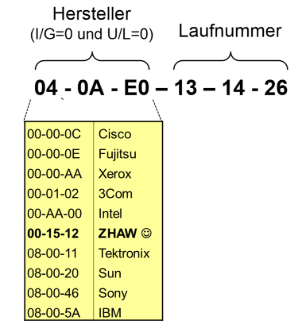
\includegraphics[width=0.4\linewidth]{images/registrierung_ieee.png}\\

    Die ersten beiden Bits des ersten Adress-Bytes klassifizieren die MAC Adresse:
    \begin{itemize}
        \item Individual / Group Bit
        \begin{itemize}
            \item 0 = individual address
            \item 1 = group address
        \end{itemize}
        \item Universally / Locally Bit
        \begin{itemize}
            \item 0 = universally administrated adress
            \item 1 = locally administrated adress
        \end{itemize}
    \end{itemize}
        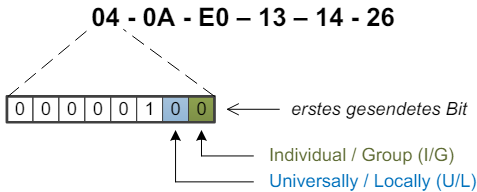
\includegraphics[width=0.6\linewidth]{images/klassifizierung_MAC_adresse.png}
\end{formula}

\begin{definition}{IEEE 802 Standards}\\
        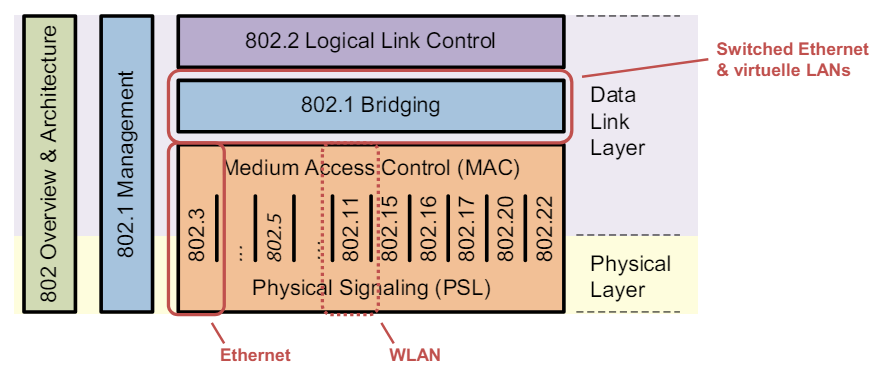
\includegraphics[width=0.8\linewidth]{images/ieee_standards.png}
\end{definition}

\begin{example2}{Ethernet Frame Format}\\
    Sie senden ein Ethernet Frame über eine 100BASE-TX Schnittstelle und beobachten auf dem Kabel folgende Bit-Sequenz:\\
    10101010 10101010 10101010 10101010 10101010 10101010\\
    10101010 10101011 00010000 00000000 01011010 11100011\\
    10011111 10000110 ...\\
    Wie lautet die MAC-Adresse (in hexadezimaler Darstellung) des Empfängers des Frames und
    wer ist der Hersteller der Ethernet-Karte dieses Empfängers?
    (Hinweis: von den einzelnen Bytes des Frames wird zuerst das LSB und am Schluss das
    MSB übertragen!)
    \begin{itemize}
        \item Zuerst 7 Bytes Präambel (10101010), dann 1 Byte SFD (10101011)
        \item 6 Bytes Destination Address: 00001000 (=08) 00000000 (=00) 01011010 (=5A) 11000111 (=C7) 11111001(=F9) 01100001(=61)
        \item MAC-Adresse: 08-00-5A-C7-F9-61, Hersteller (08-00-5A) IBM
    \end{itemize}
\end{example2}

\begin{definition}{Kollisionen}
    \begin{itemize}
        \item Bei Überlagerungen von Signalen. (Ergänzung 2 Schicht 2)
        \item Bspw. zwei Frames kommen gleichzeitig im Hub (Schicht 1) an (Minimaler Switch (Schicht 2) kann dies nicht passieren).
        \item Vollduplex: Keine Kollision da keine Spannungserhöhung (kann man prüfen).
        \item Hub / Repeater erkennt Kollisionen wenn gleichzeitig von mehreren Ports Frames empfangen werden.
    \end{itemize}
\end{definition}

\begin{formula}{Kollisionserkennung}
    können durch Überlagerung von Signalen entstehen. Kollisionen müssen erkannt werden!\\
        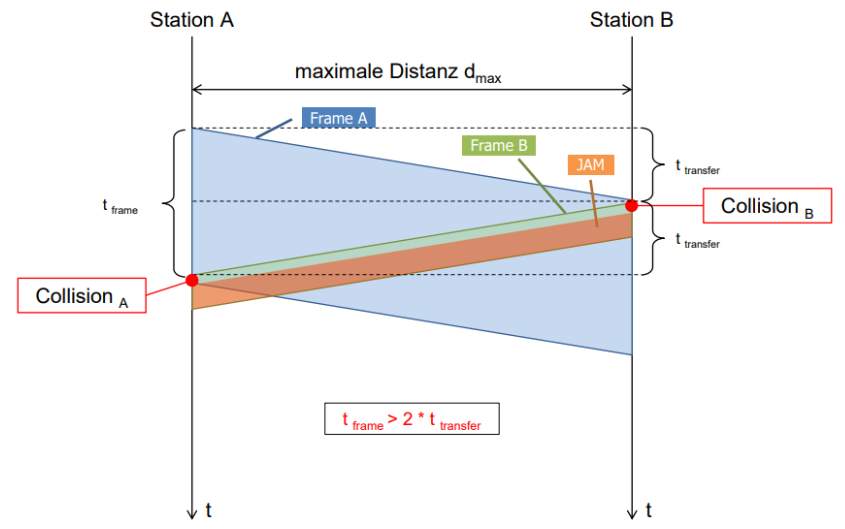
\includegraphics[width=0.9\linewidth]{images/kollisionserkennung_lan.png}\\
    Bedingungen für Kollisionserkennung:
    \begin{itemize}
        \item Ohne Repeater: $t_{frame} > 2 \cdot t_{transfer}$
        \item Mit Repeater: $t_{frame} > 2 \cdot (\sum t_{transfer} + \sum t_{forwarding})$
    \end{itemize}
    Maximale Ausdehnung eines Segments:
    $$t_{frame} = \frac{Framesize_{min}}{Bitrate}, t_{transfer} = \frac{d_{max}}{C_{Medium}}$$
    Ein Knoten kann Kollisionen nur lokal erkennen, solange er selbst am Senden ist
    $$d_{max} < \frac{1}{2} \cdot \frac{Framesize_{min}}{Bitrate} \cdot C_{Medium}, d_{max} < \frac{1}{2} \cdot \frac{576 Bit}{10 \cdot 10^6 \cdot Bit/s}$$
\end{formula}

\subsection{Switched LAN und Ethernet}

\begin{definition}{Switch/Brigde}
    \begin{itemize}
        \item Verwenden «Filtering Database».
        \item Switch lernt nur die Senderadressen nicht den Empfänger.
        \item Unbenutzte Einträge werden nach einer gewissen Zeit gelöscht.
        \item Port Mirroring möglich
    \end{itemize}
\end{definition}



\subsubsection{Ethernet Geräte (Network Gear)}

\begin{concept}{Repeater and Collision Domain}\\
    Eine Collision Domain ist ein Teilbereich eines LANs, in dem die Frames der Stationen miteinander kollidieren können.
    \begin{itemize}
        \item Erkennen von Kollisionen
        \begin{itemize}
            \item Halbduplex Collision Detection Unit
            \item Vollduplex Keine Kollisionen
        \end{itemize}
        \item Shared Medium Ethernet
        \begin{itemize}
            \item Carrier Sense Multiple Access with Collision Detection (CSMA/CD)
        \end{itemize}
        \item Normen für CSMA/CD
        \begin{itemize}
            \item Verbilligung (Thick Ethernet → Thin Ethernet)
            \item Vereinfachung (Koaxial → Twisted Pair)
            \item Leistungssteigerung (10 → 100 … 100’000 Mbit/s)
        \end{itemize}
    \end{itemize}
        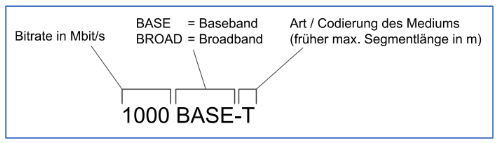
\includegraphics[width=0.75\linewidth]{images/normen_csmacd.png}
    \begin{itemize}
        \item Repeater/Hub
        \begin{itemize}
            \item Ankommendes Signal wird an alle anderen Ports weitergeleitet, regeneriert und ausgesendet. 
        \end{itemize}
    \end{itemize}
        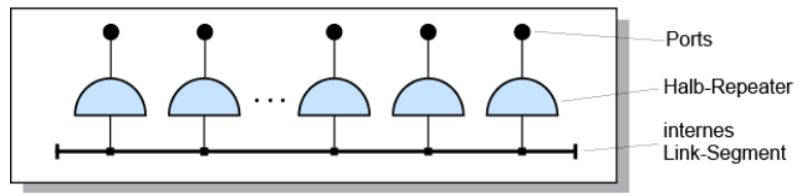
\includegraphics[width=0.75\linewidth]{images/repeater_hub.png}
\end{concept}

\begin{definition}{Repeater/Hubs im OSI Modell}
    \begin{itemize}
        \item Verstärkt ankommende Signal auf einem Port und leitet sie «in bester Qualität» weiter
        \begin{itemize}
            \item Aufgetretene Bitfehler werden ebenfalls weitergeleitet / keine Fehlererkennung
            \item Signalpegel, Signalflanken etc. sind regeneriert
        \end{itemize}
        \item Medienkonverter (elektrisch-optisch oder COAX-Twisted Pair) sind funktionell gleichwertig
    \end{itemize}
        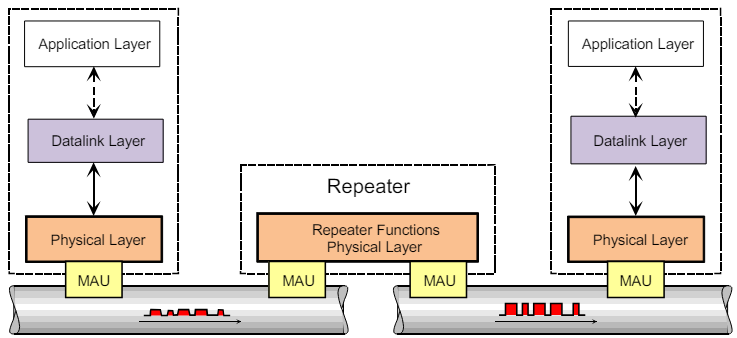
\includegraphics[width=1\linewidth]{images/repeater_hub_osimodell.png}
\end{definition}

\begin{definition}{Switch im OSI Modell}\\
    Switch arbeitet auf der Schicht 2: IEEE nennt einen Layer-2 Switch eine Bridge
    \begin{itemize}
        \item Prüft Checksumme und kann Layer-2 Adressen auswerten
        \item hat bereits seit längerem HUBs verdrängt, keine Kostenvorteile mehr
    \end{itemize}
    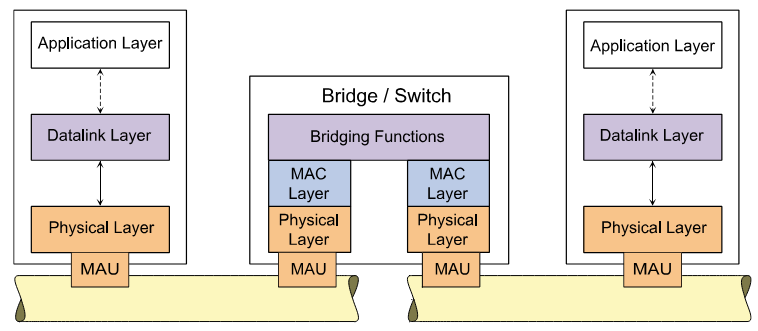
\includegraphics[width=0.8\linewidth]{images/switch_osimodell.png}
\end{definition}

\begin{definition}{Filtering Database}
    Switches verbinden LAN-Segmente\\
        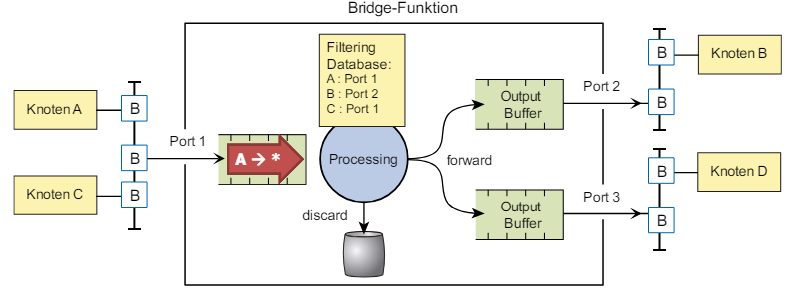
\includegraphics[width=1\linewidth]{images/filtering_database.png}    
\end{definition}

\begin{concept}{Transparente Switches}
    \begin{itemize}
        \item Bridges sollen für Endgeräte unsichtbar sein
        \item Sicht Endgerät: A und B sind direkt verbunden
        \item Konsequenz?
        \begin{itemize}
            \item Bridges dürfen Verkehr nur dann filtern, wenn sicher kein potentieller Empfänger ausgeschlossen wird
            \item «Flooding» für Broadcast und Multicast Zieladressen
            \item Unicast Verkehr kann gefiltert werden, wenn bekannt ist, über welchen Port das Ziel erreicht werden kann
        \end{itemize}
        \item Address Learning
        \begin{itemize}
            \item Aufbau und Update der Filtering Database durch Verkehrsbeobachtung (Absenderadresse)
            \item Alte Einträge werden gelöscht, wenn kein Verkehr vom Absender mehr beobachtet wird
        \end{itemize}
    \end{itemize}
\end{concept}

\begin{definition}{Bridges}\\
    Bridges verfügen über einen Mechanismus zum Erlernen von Adressen. Eine Bridge hört den Verkehr von allen Ports ab und merkt sich die Sender-Adressen aus den empfangenen Frames in der sogenannten «Filtering Database». Diese beinhaltet für jede bekannte Mac-Adresse das Bridge-Port, über welches der zugehörige Knoten erreichbar ist. Unbenutzte Einträge in der Filtering Database werden nach einer gewissen Zeit automatisch gelöscht. \\
    Diese Verarbeitung benötigt etwas Zeit, ist aber dennoch vorteilhaft, da das Paket nur an die richtige Collision Domain geschickt wird.
\end{definition}

\begin{definition}{Multi-Port-Bridges}
    \begin{itemize}
        \item Daten werden ausschliesslich an den richtigen Port weitergeleitet.
        \item Standard-Komponente zur Kopplung von Segmenten
        \item Werden als Ethernet-Switch bezeichnet
    \end{itemize}
\end{definition}

\begin{concept}{Broadcast and Collision Domain}\\
    Eine Collision Domain (CD) besteht aus mit Repeatern zusammengeschlossenen Segmenten.
    \begin{itemize}
        \item Max. halb so lange wie die Ausdehnung des kürzesten Frames
    \end{itemize}
    Ein virtuelle LAN bildet eine Broadcast Domain. Das heisst die Grenzen für die Verteilung der
    Broadcast-Frames. 
\end{concept}

\begin{definition}{Bridges: Arbeitsweise eines 4-Port Switches}\\
        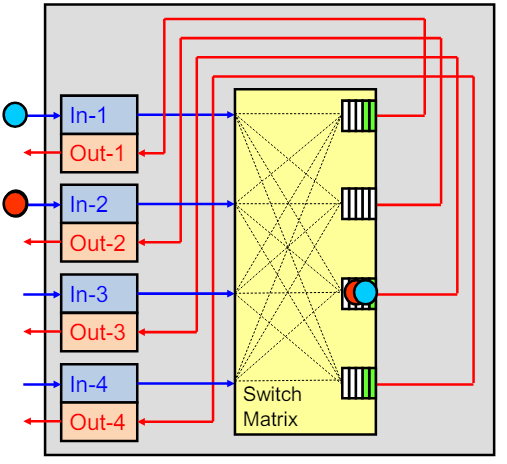
\includegraphics[width=0.5\linewidth]{images/bridges_4portswitch.png}
\end{definition}

\begin{KR}{Weg/Zeit-Diagramm für das Senden eines Frames}\\
    Gesamtübertragungszeit (Latenz): $t_{frame} + t_{transfer}$\\
    $t_{forwarding}$ kann verlängert werden um eine Verarbeitungszeit zu ermöglichen\\
        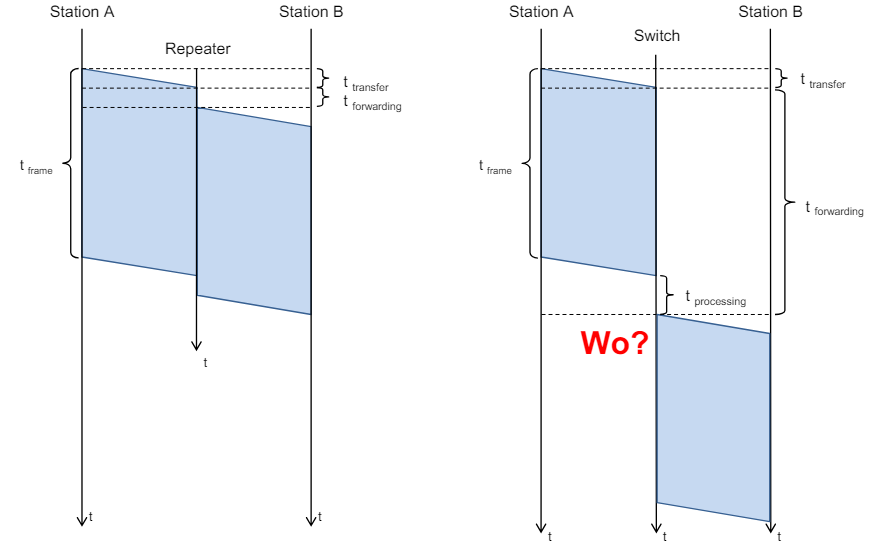
\includegraphics[width=1\linewidth]{images/weg_zeit_senden_frame.png}
\end{KR}

\begin{definition}{Übersicht Netzwerkgeräte im LAN}\\
        \includegraphics[width=1\linewidth]{images/netzwerkgeräte_LAN.png}
\end{definition}

\subsection{Redundanz (Spanning Tree)}

\begin{concept}{Spanning Tree Algorithmus}\\
    Redundante Pfade schaffen Probleme!!
    \begin{itemize}
        \item Ziel: Alle Segmente in einer loop-freien Topologie verbinden
        \item Idee:
        \begin{itemize}
            \item Root-Bridge auswählen (willkürliche, aber eindeutige Wahl) 
            \begin{itemize}
                \item Auswahl ist vom Bridge-Identifier abhängig
                \item Bridge Identifier besteht aus einer wählbaren Priorität und der MAC Adresse
            \end{itemize}
            \item Ausgehend von der Root einen Baum aufbauen
            \item Redundante Pfade sperren
            \item alle Knoten werden genau einmal verbunden
        \end{itemize}
    \end{itemize}
        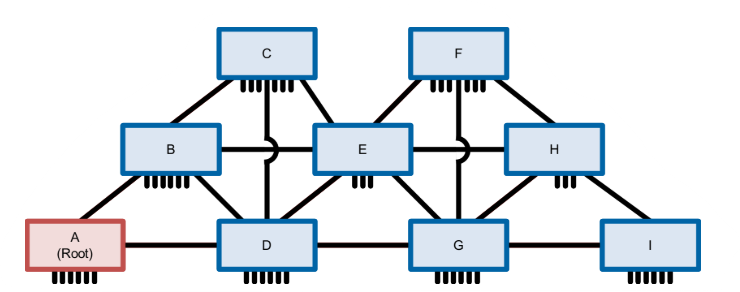
\includegraphics[width=0.6\linewidth]{images/spanning_tree_idee.png}\\
    E wäre theoretisch besser geeignet als Root-Bridge
\end{concept}

\begin{KR}{Spanning Tree Algorithmus}
    Initialisierung
    \begin{itemize}
        \item Alle Ports für Nutzdaten blockiert
        \item Annahme: «Ich bin Root»
        \item Austausch BPDUs mit Nachbarn
    \end{itemize}
    Aufbau des Spanning Tree
    \begin{itemize}
        \item Aufdatieren der Info zu Root (kleinste ID) und Pfadkosten zu dieser
        \item Austausch aufdatierter BPDUs bis Konvergenz
    \end{itemize}
    Setzen der Port Roles
    \begin{itemize}
        \item Freigeben for Nutzdaten von
        \begin{itemize}
            \item Root-Ports (Empfang der «besten» BPDU)
            \item Designated-Ports (Gegenstück zu Root-Ports)
        \end{itemize}
        \item Alle anderen Ports bleiben blockiert (Discarding)
    \end{itemize}
        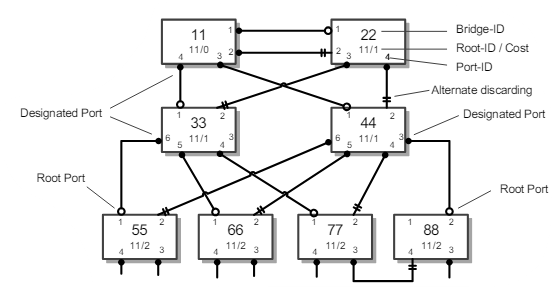
\includegraphics[width=0.75\linewidth]{images/spanning_tree_algorithmus.png}\\
        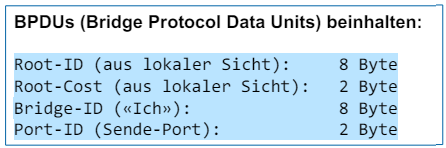
\includegraphics[width=0.5\linewidth]{images/bdpus.png}
\end{KR}

\subsection{Virtuelle LANs und Quality of Service}

\begin{definition}{VLAN}
    Mithilfe von virtuellen LAN kann ein grosses Netz in unabhängige logische Netze aufgeteilt werden. Jedes Switch-Port kann einem beliebigen VLAN zugeordnet werden.\\
    Trunk Links sind Teil von mehreren VLANS. Auf den Trunk Links müssen Frames der verschiedenen VLANs eindeutig gekennzeichtet werden!\\
        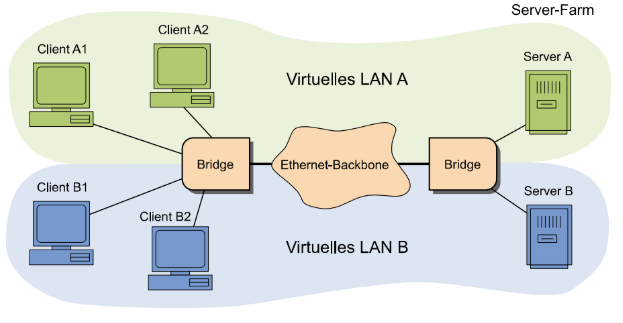
\includegraphics[width=1\linewidth]{images/vlan.png}\\
    Trunk = Tagged, Access = Untagged
\end{definition}

\begin{definition}{VLAN Tag}
    \begin{itemize}
        \item VLAN-ID im VLAN-Tag wird zur Zuordnung verwendet
        \item Priority Code Point ermöglicht die Priorisierung gewisser Applikationen
        \item Discard Eligibility Indicator 0 → Frame wird bei Engpässen zuerst verworfen
        \item VLAN Tagging erfolgt oft beim Eintritt/Austritt ins Netz
        \item Vorteile:
        \begin{itemize}
            \item Transparent (unsichtbar) für Endgeräte
            \item VLAN Konfiguration nur im Netz
            \begin{itemize}
                \item Einfache zentrale Konfiguration
                \item Einfaches Anpassen der Konfiguration
            \end{itemize}
        \end{itemize}
    \end{itemize}
\end{definition}

\begin{formula}{VLAN Tagging}\\
    Erweiterung des Ethernet Headers durch einen VLAN-Tag
    \begin{itemize}
        \item Der Type 0x8100 bedeutet, dass das Frame «getagged» ist
        \item Ein 12 Bit Identifier (VLAN-ID, VID) besagt, welchem VLAN das Frame angehört
        \item Die 3 Bit des Priority Code Point (PCP) erlauben, das Frame mit einer Priorität zu versenden
        \item Mit dem Drop Eligibility Indicator (DEI) werden Frames markiert, die bei Überlastsituationen zuerst verworfen werden sollen
    \end{itemize}
    Die maximalen Nutzdatenlänge bleibt erhalten, der Ethernet Frame wird 4 Bytes länger
    \begin{itemize}
        \item VLANs können transparent eingesetzt werden
    \end{itemize}
        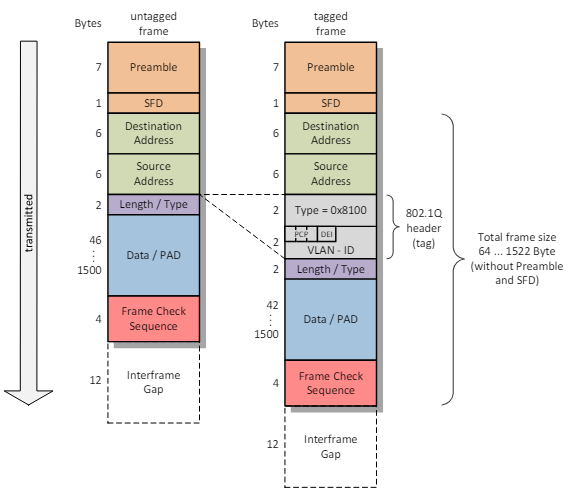
\includegraphics[width=1\linewidth]{images/vlan_tagging.png}
\end{formula}

\begin{concept}{Quality of Service (QoS}\\
    Quality of Service: Priorisierung aufgrund der PCP-Werte (0 .. 7)
    \begin{itemize}
        \item Erlaubt Unterstützung verschiedener Verkehrsklassen im Layer 2, wie
        \begin{itemize}
            \item Voice (< 10 ms Latenz)
            \item Video (< 100 ms Latenz)
            \item Best Effort Daten
            \item Background Daten
        \end{itemize}
        \item Jeder Switch-Port verfügt über mehrere Ausgangs-Queues (bis zu 8)
        \begin{itemize}
            \item Frames können sich im Switch überholen
            \item Verschiedene Priorisierungs-Strategien möglich, im einfachsten Fall «Strict Priority»
            \begin{itemize}
                \item Prio 7 vor Prio 6 ... ... vor Prio 0
            \end{itemize}
        \end{itemize}
    \end{itemize}
        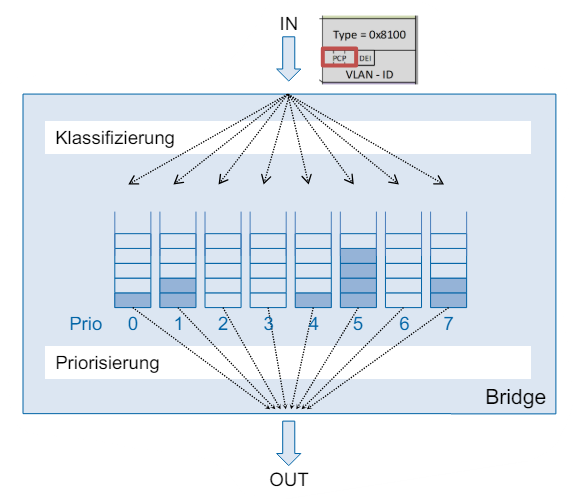
\includegraphics[width=0.7\linewidth]{images/qualityofservice.png}
\end{concept}

\begin{theorem}{Switched LANs: Merkmale von Switches/Bridges}\\
        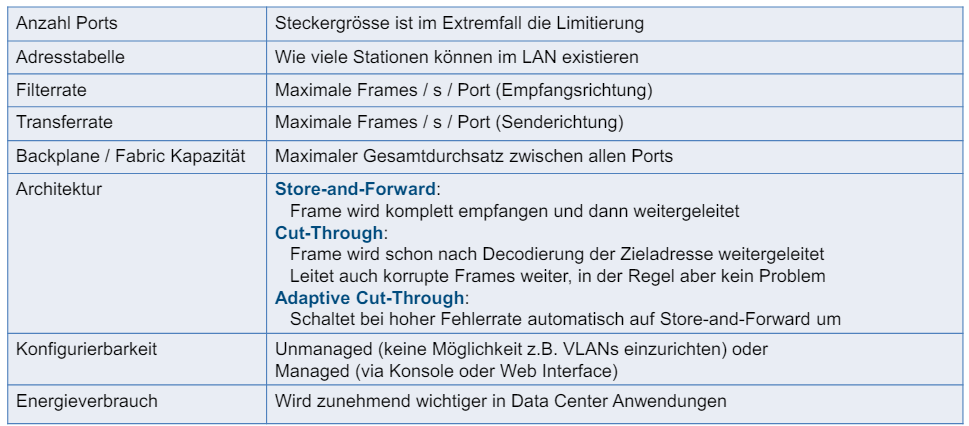
\includegraphics[width=1\linewidth]{images/merkmale_switches_bridges.png}
\end{theorem}

\textbf{UNTERSCHIEDE BRIDGES UND SWITCHES}

\begin{concept}{Switched LAN Monitoring}
    Hub/Multiport Reader
    \begin{itemize}
        \item Pro
        \begin{itemize}
            \item Alle Daten sind auf allen Ports sichtbar
        \end{itemize}
        \item Con
        \begin{itemize}
            \item Verfälscht die Situation völlig
            \item Nur Half Duplex Betrieb für A und B möglich
        \end{itemize}
    \end{itemize}
    Tap/Probe
    \begin{itemize}
        \item Pro
        \begin{itemize}
            \item Sehr detaillierte low-level Analyse möglich
        \end{itemize}
        \item Con
        \begin{itemize}
            \item Kosten
            \item Veränderung des Netzwerkes (Latenz)
        \end{itemize}
    \end{itemize}
\end{concept}

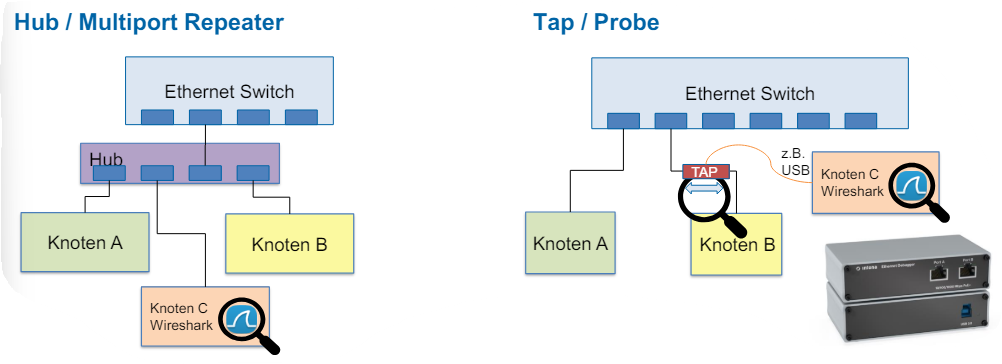
\includegraphics[width=1\linewidth]{images/switched_lan_monitoring.png}

\begin{concept}{Port Mirroring}
    Managed Switches unterstützen eine Vielzahl Diagnosefunktionen
    \begin{itemize}
        \item Statistik Zähler pro Port: Anzahl Rx und Tx Frames, FCS-Fehler, zu lange Frames, ...
    \end{itemize}
    Port-Mirroring leitet Daten zusätzlich auf einen anderen Port um
    \begin{itemize}
        \item Konfigurationsoptionen herstellerabhängig
        \begin{itemize}
            \item Kompletter Port (Rx plus Tx), oder selektiv Port Nummer(n) und Richtung
        \end{itemize}
    \end{itemize}
        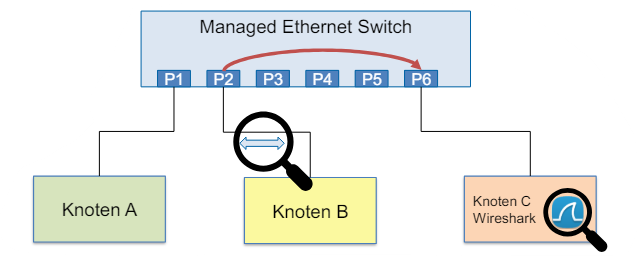
\includegraphics[width=0.6\linewidth]{images/port_mirroring.png}
\end{concept}

\subsubsection{Ethernet Systeme}

\begin{theorem}{Bezeichnungs-Schema}\\
    Jede im Standard IEEE 802.3 definierte Technologie hat einen dreiteiligen Namen, der ihre Eigenschaften beschreibt\\
    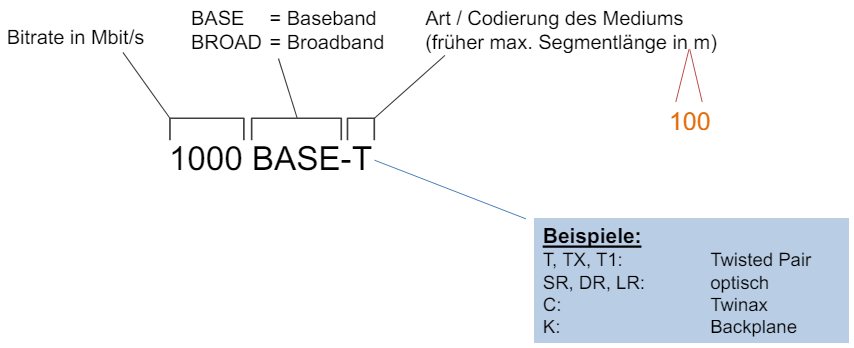
\includegraphics[width=0.9\linewidth]{images/ethernet_bezeichnungsschema.png}\\
    10BASE... heisst 10Mbps, 10GBASE heisst 10Gbps, usw.
\end{theorem}

\begin{definition}{Topologie aller Twisted-Pair-Ethernet}
    \begin{itemize}
        \item Stern-Topologie mit mehreren Stationen an einem Ethernet Switch
        \item Mehrere Switches erweitern Topologie zu einem Baum
        \item Für Twisted Pair (10 Mbit/s .. 10 Gbit/s) gilt in der Regel:
        \begin{itemize}
            \item 4 verdrillte Aderpaare (für < 1 Gbit/s auch 2)
            \item Maximale Segmentlänge 100m
            \item RJ45 Stecker
        \end{itemize}
        \item Allenfalls vermascht für Redundanz
    \end{itemize}
        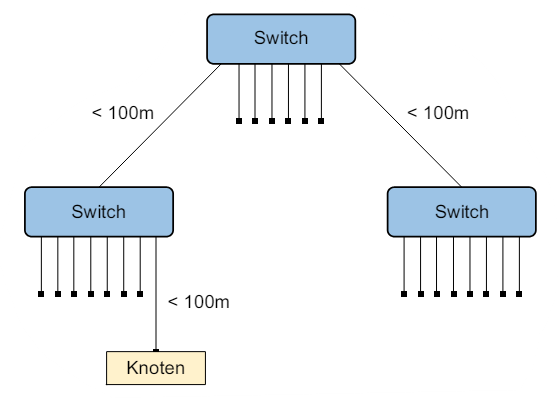
\includegraphics[width=0.6\linewidth]{images/topologie_twistedpair_ethernet.png} 
\end{definition}

\begin{concept}{Autonegation}
    \begin{itemize}
        \item Konzept
        \begin{itemize}
            \item Ermittlung der besten Betriebsart durch Austausch der Leistungsmerkmale zweier Netzwerkkomponenten.
            \item beruht auf Fast Link Pulses
        \end{itemize}
        \item Link Pulses
        \begin{itemize}
            \item NLP = Link Presence Detection
            \item FLP = Autonegotiation, Autopolarity
        \end{itemize}
    \end{itemize}
        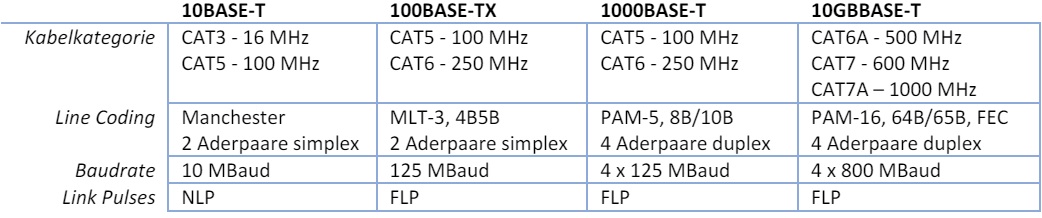
\includegraphics[width=1\linewidth]{images/ethernet_systeme.png}\\
        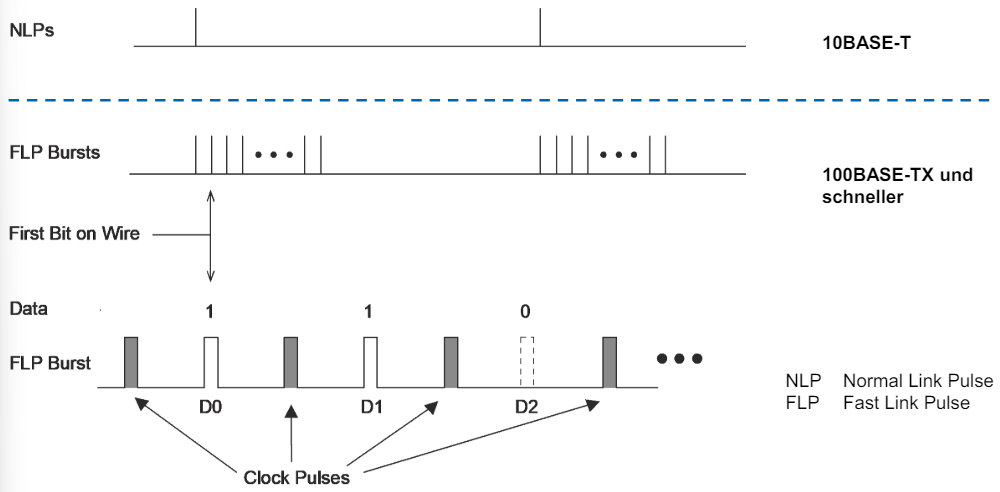
\includegraphics[width=1\linewidth]{images/autonegation.png}
\end{concept}

\begin{concept}{Leitungscodierung}\\
    NRZI-Codierung (Non Return to Zero Inverted), kombiniert mit MLT-3\\
        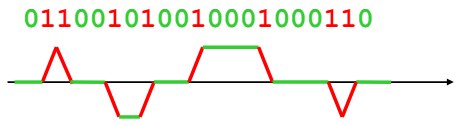
\includegraphics[width=0.5\linewidth]{images/leitungscodierung.png}\\
    MLT-3 = Multi-Level Transmit - Ternary
\end{concept}

\begin{formula}{GBASE-T}\\
        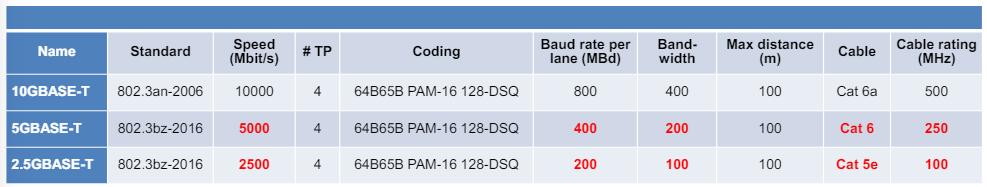
\includegraphics[width=1\linewidth]{images/GBASE-T.png}
\end{formula}

\begin{concept}{Twisted Pair Ethernet Evolution Übersicht}\\
        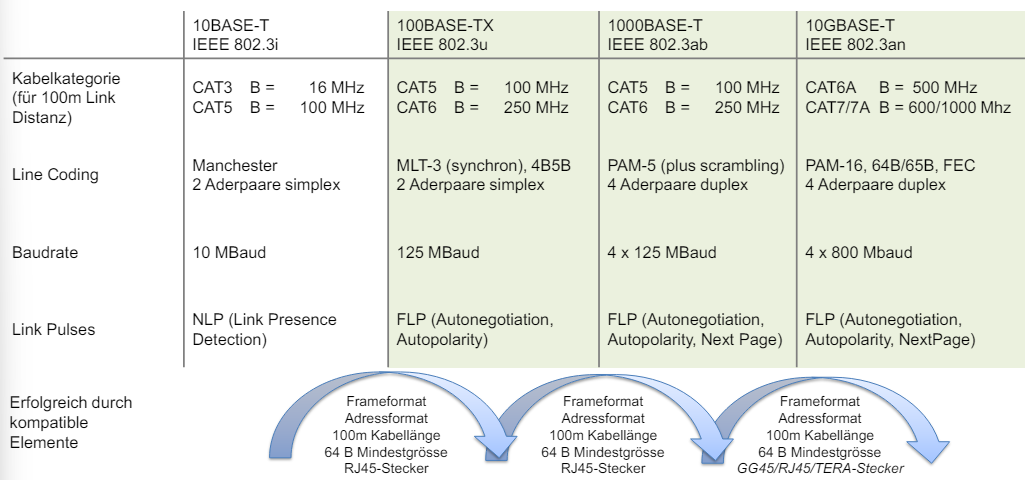
\includegraphics[width=1\linewidth]{images/twistedpair_ethernet_evolution.png}
\end{concept}

\begin{KR}{Key Takings LAN/Ethernet Basics}
    \begin{itemize}
        \item LANs waren historisch räumlich kleine Netze, die verschiedene Geräte verbinden und in welchen Daten mit hoher Geschwindigkeit übertragen werden
        \item LAN-Topologien sind Bus, Linie, Ring, Stern, Baum und vermaschte Strukturen
        \item IEEE hat in den Normen 802 eine Reihe von Standards für LAN und MAN aufgestellt
        \item Alle Ethernet Varianten
        \begin{itemize}
            \item Definieren die physikalische und Teile der Sicherungsschicht
            \item verwenden das gleiche Frame-Format, das auch in allen später entwickelten Ethernet/802.3 -Varianten verwendet wird
            \item MAC-Adressen der Länge 6 Bytes identifizieren Ethernet Geräte
        \end{itemize}
        \item 10BASE-T ist bereits sehr alt, kann aber einfach beobachtet werden
        \begin{itemize}
            \item Manchester Codierung, Unterstützung von Repeatern/Hubs
        \end{itemize}
        \item Switches (Bridges) arbeiten transparent (unsichtbar) auf dem Data Link Layer und schliessen mehrere Segmente zu einem LAN zusammen
        \begin{itemize}
            \item Bridges leiten (Address Learning) Frames nur dorthin weiter, wo sie empfangen werden müssen $\longrightarrow$ Lastreduzierung und Erhöhung der effektiv nutzbaren Kapazität
        \end{itemize}
    \end{itemize}
\end{KR}

\begin{KR}{Key Takings Ethernet-Technologie und -Systeme}
    \begin{itemize}
        \item Mit gemanagten Switches/Bridges kann ein physikalisches LAN in mehrere virtuelle LANs (VLAN) mit separaten Broadcast Domains aufgeteilt und Prioritäten unterstützt werden
        \item Port Mirroring ist ein mögliches Verfahren zur Verkehrsbeobachtung und Fehlersuche in Switched Ethernet
        \item Redundanz wird ermöglicht
        \begin{itemize}
            \item durch die „künstliche“ Reduktion der Topologie au eine aumstruktur durch Spanning Tree Algorithmen
        \end{itemize}
        \item Kompatibilität (10)/100/1000BASE-T wird erreicht durch
        \begin{itemize}
            \item Beibehaltung von Frame Format und Schnittstelle zwischen PHY und MAC
            \item Autonegotiation mittels FLP bursts / NLP
        \end{itemize}
        \item PHY Codierung ist unterschiedlich (Scrambled NRZ/MLT-3 mit 4 5 Codierung, …)
        \begin{itemize}
            \item Höhere Datenrate → höhere Ansprüche an die Signalverarbeitung und Algorithmen im PHY
            \item Massnahmen zur Reduktion von Maximaler Signalfrequenz und EMV Pegeln werden mit steigender Datenrate immer wichtiger
        \end{itemize}
        \item Zur Zeit dominieren
        \begin{itemize}
            \item Geswitchte 100BASE-TX oder 1000BASE-T Systeme, die oft gemeinsam in einem LAN betrieben werden
            \item Geswitchter Vollduplex Betrieb (mikrosegmentiertes LAN)
        \end{itemize}
    \end{itemize}
\end{KR}

